\section{Description}
The DBELA methodology is a nonlinear static analytical for the seismic risk assessment of buildings. This method arises as a solution to the lack of a methodology capable of combining good correlation with damage, easy to calibrate, transparent, theoretically robust and with a full probabilistic treatment of the variables. As a continuation of the urban assessment methodology proposed by \citet{Calvi1999} in which principals of structural mechanics and seismic response of buildings are used to estimate the seismic vulnerability of classes of buildings, \citet{Pinhoetal2002} presents for the first time a displacement-based earthquake loss assessment methodology.  \citet{GlaisterPinho2003} carried out further developments on the equations and \citet{Crowleyetal2004} adapted the methodology to assess RC buildings in a more practical way. 
The introduction of a probabilistic framework capable of considering the uncertainty on the demand and capacity was proposed by \citet{Crowleyetal2006} and in \citep{Baletal2010} new contributions were added to the methods such as the inclusion of new failure mechanisms and building typologies or the evaluation and quantification of the uncertainty of several parameters.
The most up to date version of this methodology is described herein highlighting the building typologies that can be considered, the formulas that are being employed and how the uncertainty is being taking into account.

\section{Procedure}
This methodology is strongly based on the Displacement-based Design rules introduced by  \citet{Priestley1997} and \citet{Priestleyetal2007} in which a multiple degree of freedom (MDOF) structure is converted in to an equivalent structure with a single degree of freedom (SDOF). Then, the following parameters need to be computed: 

\begin{itemize}
\item Limit state displacement capacity;
\item Limit state ductility values;
\item Limit state periods;
\item Displacement demand;
\end{itemize}

Once these parameters are obtained, the displacement capacity of the first limit state is compared with the respective demand. If the demand exceeds the capacity, the next limit states need to be checked successively, until the demand no longer exceeds the capacity and the building damage state can be defined. If the demand also exceeds the last limit state, the building is assumed to have collapsed. This procedure can be schematically seen in Figure \ref{fig:dbela_procedure} in which the capacity for each limit state is being represented by $\Delta_{LS}$ and the associated demand by $S_{di}$. In this example, the demand exceeds the capacity in first and second limit state but not on the third limit state which allocates the building in the third damage state.

\begin{figure}[ht]
\centering
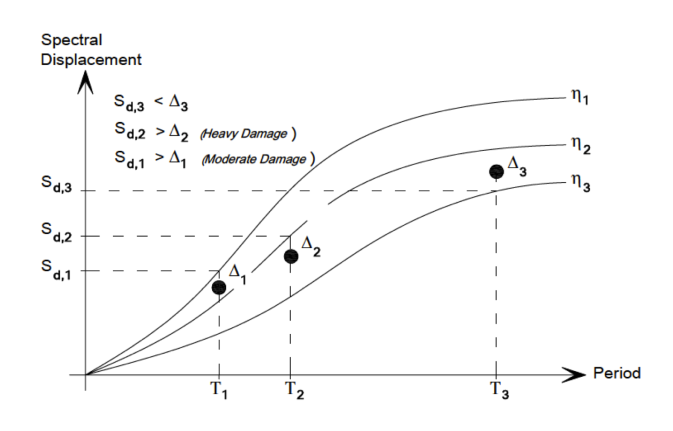
\includegraphics[width=10cm,height=6cm]{./Figures/Part_Risk/dbela_procedure.eps}
\caption{Comparison between the capacity for each limit state and the associated demand \citep{Baletal2010}.}
\label{fig:dbela_procedure}
\end{figure}

Each displacement capacity ($\Delta_{LS}$) is computed based on the secant stiffness at the respective limit state and a level of equivalent viscous damping, representative of the combined elastic damping and hysteretic energy absorbed during the inelastic response \citep{Baletal2010}. The respective displacement demand can either be calculated using an over-damped spectrum or using a ground motion prediction equation (GMPE). In both cases, the displacement demand is computed for the period at each limit state and modified by a correction factor $\eta_i$, representative of the equivalent viscous damping and limit state ductility. The formulas that are employed to compute the previously described parameters can vary based on the type of structure. The following section presents the most of to date equations for each building typology currently covered by the methodology.

\section{Building typologies}
The building typologies that can be assess through this method were grouped into Reinforced Concrete and Masonry structures. A description of the whole displacement-based procedure for each building typology can be found in \citep{Baletal2010}. For what concerns this document, it will be presented the most important formulas and parameters. The following list describes the symbols that will be used on the aforementioned formulas:

\begin{table}[ht]
\caption{Summary of the symbols}
\centering
\begin{tabular}[ht]{ll}
Symbol & Description \\[0.5ex]\hline
$\Delta_{Sy}$ & Limit state 1 (yield) structural displacement capacity\\
$\Delta_{SLSi}$ & Limit state i (post-yield) structural displacement capacity\\ 
$ef_h$ & Effective height coefficient\\
$\epsilon_y$ & Yield strain of reinforcement steel\\
$\epsilon_{C\left({LS_i}\right)}$ & Limit state i (post-yield, spalling/crushing) concrete strain\\ 
$\epsilon_{S\left({LS_i}\right)}$ & Limit state i (post-yield)  reinforcement steel strain\\ 
$h_c$ & Depth of column section\\
$h_s$ & Height of ground-floor storey\\
$h_b$ & Height of beam\\
$l_b$ & Length of beam\\
$T_y$ &Yield period of vibration\\
$T_{LS_i}$ & Limit state i (post-yield) period of vibration
\end{tabular}
\label{table:SymbolTable}
\end{table}

\subsection{Reinforced Concrete Buildings}

\subsubsection{Frames with emergent or embedded beams}
A great proportion of the residential and commercial Mediterranean buildings are constructed in reinforced concrete with masonry infills. Such buildings tend to have a beam-column frame structural behavior in which the masonry panels might not have a robust connection to the frame. These structures can either follow a joist-slab-column system in which the slabs are built between embedded beams with a thin layer of concrete on the top of the hollow bricks (embedded beams), or another construction typology in which the beams depth are considerably greater than the slab depth (emergent bems). In the first construction approach the columns tend to be larger due to the fact that the distribution of the moments around the joint required the column to withstand higher levels of stress \citep{Baletal2010}. In Figures \ref{fig:beam_sections} and \ref{fig:beam_construction} the differences between these two types of construction can be seen.

\begin{figure}[ht]
\centering
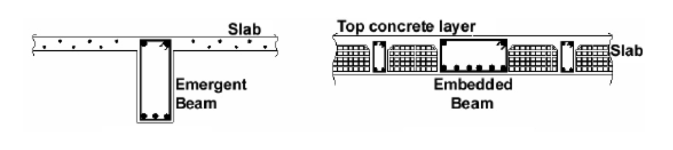
\includegraphics[width=14cm,height=2.5cm]{./Figures/Part_Risk/beam_types_sections.eps}
\caption{Cross section of emergent beam (left) and embedded beam (right)\citep{Baletal2010}.}
\label{fig:beam_sections}
\end{figure}

\begin{figure}[ht]
\centering
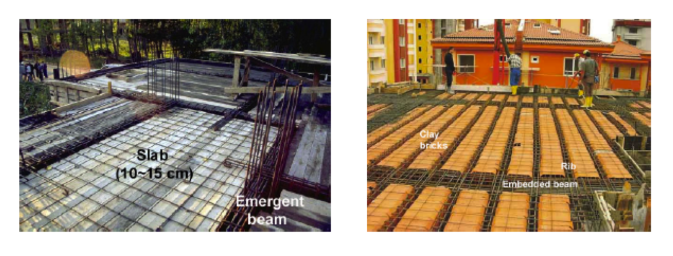
\includegraphics[width=14cm,height=5cm]{./Figures/Part_Risk/beam_types_construction.eps}
\caption{Construction application of emergent beam (left) and embedded beam (right)\citep{Baletal2010}.}
\label{fig:beam_construction}
\end{figure}

\paragraph{Bare frame structures}

The procedure  proposed by \citep{Crowleyetal2006} for bare frames have been used, with the exception of the equations to estimate the deformed shape that were replaced by the ones presented by \citep{Priestleyetal2007}. The displacement capacity and ductility values for each limit state depend on the failure mechanism that will affect the structure. Two response mechanisms are considered within the methodology: beam-sway and column-sway, as described by \citet{PaulayPriestley1992}. Thus, to compute the yield (first limit state) displacement capacity for beam-sway and column-sway bare frames, the following formulae can be used respectively:

\begin{equation}
\Delta_{Sy}=0.50\delta_{eff}H_T\epsilon_y\frac{l_b}{h_b}
\end{equation}

\begin{equation}
\Delta_{Sy}=0.43\delta_{eff}H_T\epsilon_y\frac{h_s}{h_c}
\end{equation}

The post-yield displacement capacity for the second and third limit state are calculated by adding a plastic displacement component to the yield displacement, obtaining the following formulae:

\begin{equation}
\Delta_{Sy}=0.50\delta_{eff}H_T\epsilon_y\frac{l_b}{h_b}+0.5(\epsilon_{C\left({LS_i}\right)}+\epsilon_{S\left({LS_i}\right)}-1.7\epsilon_y)\delta_{eff}HT
\end{equation}

\begin{equation}
\Delta_{Sy}=0.43\delta_{eff}H_T\epsilon_y\frac{l_b}{h_b}+0.5(\epsilon_{C\left({LS_i}\right)}+\epsilon_{S\left({LS_i}\right)}-2.14\epsilon_y)h_s
\end{equation}

The effective height coefficient  $\delta_{eff}$ in the above formulae can be compute for beam-sway frames using equations: 

\begin{equation}
for \ \ n\leq 4 \ \ \delta_{eff}=H_i/H_T
\end{equation}

and

\begin{equation}
for \ \ n> 4 \ \ \delta_{eff}=(4/3)(H_i/H_T)(1-H_i/(4H_T))
\end{equation}
%\hfill \\
Where $H_i$ stands for the height of the storey, $H_T$ stands for the total height of the building and $n$ stands for the number of storeys. 
Regarding column-sway frames, the equation first proposed by \citet{Priestley1997}  and then adapted by  \citet{GlaisterPinho2003} can be used:
\begin{equation}
\delta_{eff}=0.67-0.17\frac{\mu_{LSi}-1}{\mu_{LSi}}
\end{equation}
It should be noted that the ductility values $\mu_{LSi}$ for column-sway frames also depend on the $\delta_{eff}$ as it will be shown ahead. In this case, an iterative procedure needs to be employed. However, in order to overcome this issue, \citet{GlaisterPinho2003} proposed a similar formula in which the ductility was replaced by the steel strain:
%
\begin{equation}
\delta_{eff}=0.67-0.17\frac{\epsilon_{LSi}-\epsilon_y}{\epsilon_{LSi}}
\end{equation}
\vspace{5mm}
%
Within OpenQuake, both approaches have been implemented and users can choose which one should be followed.  
Each limit state ductility value $\mu_{LSi}$ for beam-sway and column-sway frames can be obtained by dividing the displacement capacity of the respective limit state  by the yield displacement capacity, as shown respectively in the following equations:
%
\begin{equation}
\mu_{LSi}=1+\frac{(\epsilon_{C\left({LS_i}\right)}+\epsilon_{S\left({LS_i}\right)}-1.7\epsilon_y)h_b}{\epsilon_yl_b}
\end{equation}
\begin{equation}
\mu_{LSi}=1+\frac{(\epsilon_{C\left({LS_i}\right)}+\epsilon_{S\left({LS_i}\right)}-2.14\epsilon_y)h_c}{0.86\delta_{eff}H_T\epsilon_y}
\end{equation}
%\hfill \\
Regarding the period for each limit state, different equations have been proposed for bare frames with emergent beams or embedded beam. For the former, \citet{CrowleyPinho2004} suggested a yield period equal to $0.1H_T$ while for the later, as presented by \citet{Kumar2008} and verified by \citet{Baletal2010}, a yield period equal to $0.12H_T$ can be assumed. As for the second and third limit state period, if the post-yield stiffness ratio can be neglected, the following formula proposed by  \citet{Crowleyetal2006} can be employed:

\begin{equation}
T_{LS}=T_y\sqrt{\mu_{LS}}
\label{eq:Post-yieldPeriod}
\end{equation}

\paragraph{Infilled frame structures}
 
The presence of masonry infill walls increases the strength of the building and slightly decreases the displacement capacity. In order to incorporate the decrease on the displacement capacity on the respective equations, a parameter $\beta_{i}$ which varies between 0 and 1 has been added to the formulae used for bare frame structures. Thus, the following equations for beam-sway and column-sway can be used respectively:

\begin{equation}
\Delta_{Sy}=\left[0.50\delta_{eff}H_T\epsilon_y\frac{l_b}{h_b}\right]\beta_1+\left[0.5(\epsilon_{C\left({LS_i}\right)}+\epsilon_{S\left({LS_i}\right)}-1.7\epsilon_y)\delta_{eff}H_T\right]\beta_2
\end{equation}

\begin{equation}
\Delta_{Sy}=\left[0.43\delta_{eff}H_T\epsilon_y\frac{l_b}{h_b}\right]\beta_1+\left[0.5(\epsilon_{C\left({LS_i}\right)}+\epsilon_{S\left({LS_i}\right)}-2.14\epsilon_y)h_s\right]\beta_2
\end{equation}

\citet{Baletal2010} ran several displacement-based adaptive pushover analysis on a set of mediterranean buildings with the purpose of evaluating the decrease on the displacement capacity for each limit state. Using these results, a mean $\beta_{i}$ have been proposed as given in Table  \ref{table:MeanBeta}.

\begin{table}[ht]
\caption{Mean $\beta_i$ values}
\centering
\begin{tabular}[ht]{cccc}
Infilled Case & $LS1(\beta_1)$ & $LS2(\beta_2)$ & $LS3(\beta_2)$ \\[0.5ex]\hline
Embedded beam frames & 0.60 & 0.62 & 0.49\\
Emergent beam frames & 0.52 & 0.46 & 0.28\\
\end{tabular}
\label{table:MeanBeta}
\end{table}

As far as period-height relationship, the increase in strength causes a decreases on the yield period. For emergent beam infilled frames, \citet{CrowleyPinho2006} suggested a yield period equal to $0.055H_T$ while for embedded beam infilled frames, \citet{Kumar2008} proposed a yield period equal to $0.06H_T$. Regarding the post-yield periods, the same procedure suggested for bare frame structures can be employed (see equation \ref{eq:Post-yieldPeriod}).

\subsubsection{Frame-wall structures}

Often buildings have both frames and walls contributing to the seismic resistance, as illustrated in Figures  \ref{fig:Dual_frame_wall_plan} and  \ref{fig:Dual_frame_wall_front}.

\begin{figure}[ht]
\centering
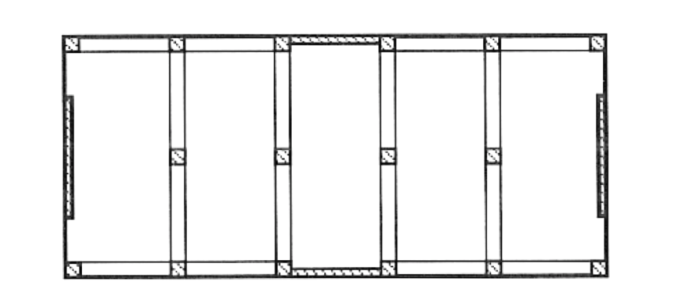
\includegraphics[width=8cm,height=3cm]{./Figures/Part_Risk/Dual_frame_wall_plan.eps}
\caption{Plan view of a dual wall-frame structure \citep{Priestleyetal2007}.}
\label{fig:Dual_frame_wall_plan}
\end{figure}

\begin{figure}[ht]
\centering
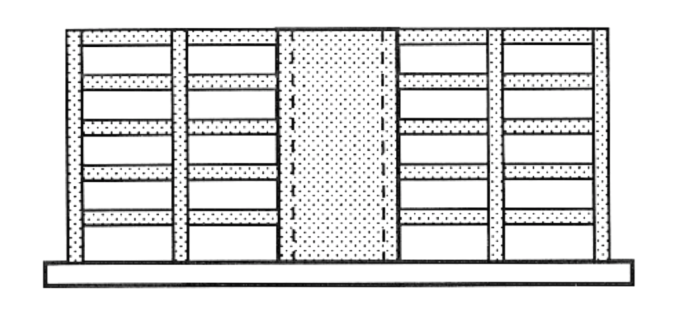
\includegraphics[width=8cm,height=3cm]{./Figures/Part_Risk/Dual_frame_wall_front.eps}
\caption{Front view of a dual wall-frame structure \citep{Priestleyetal2007}.}
\label{fig:Dual_frame_wall_front}
\end{figure}

As far as the DBELA methodology concerns, the procedure defined by \citet{Sullivanetal2006} and \citet{Priestleyetal2007} was adopted. Thus, assuming that a shear-away failure mechanism is not likely to occur, the displacement capacity can be given by the following formulae:

\begin{equation}
for \ \ H_i\leq H_{CF} \ \ \Delta_{yi}=2\epsilon_y/l_w(H_i^2/2-H_i^3/(6H_{CF}))
\end{equation}

\begin{equation}
for \ \ H_i\ge H_{CF} \ \ \Delta_{yi}=2\epsilon_y/l_w(H_{CF}H_i/2-H_{CF}^2/6))
\end{equation}

\begin{equation}
\Delta_{LS2}=\Delta_{yi}+(0.0174/l_w-2\epsilon_y/l_w)L_p+H_i
\end{equation}

\begin{equation}
\Delta_{LS3}=\Delta_{yi}+(0.0720/l_w-2\epsilon_y/l_w)L_p+H_i
\end{equation}
%\hfill\\

Where $H_{CF}$ stands for the height of the contra-flexure, amd $L_p$ is the plastic hinge length given by the following equation:

\begin{equation}
L_p=kH_CF+0.1l_w+0.0022f_yd_{bl}
\end{equation}

Where $l_w$ is the wall lenght, $d_bl$ is the diameter of the vertical rebars and $k$ is equal to $0.2(f_u/f_y-1)\leq 0.08$ where $f_u$ and $f_y$ are equal to the the ultimate and yield strength of the steel respectively.

The estimation of the effective height for dual frame-wall structures proved to be more challenging due to the fact that it is common to occur both beam- and column-sway mechanisms simultaneously. For a pure beam-sway mechanism, an effective height ratio of 0.7 can be used while for a pure column-sway mechanism, an effective height ratio equal to 0.5 can be assumed \citep{Priestleyetal2007}. \citet{Baletal2010} conducted several analysis with the purpose of estimating the contribution of the frames to the total base shear (represenred by $\beta_{MF}$ and the relationship between the total height of the building and the respective effective and contra-flexure height. A normal distribution was fit to these values and the mean and coefficient of variation are presented in table \ref{table:FrameWallParameters}.

\begin{table}[ht]
\caption{Parameters for the assessment of dual wall-frame structures}
\centering
\begin{tabular}[ht]{cccc}
Parameter & Mean & COV & Lower-Upper Bounds \\[0.5ex]\hline
$\beta$ & 0.12 & 0.6 & 0.04 - 0.40   \\
$H_{CF}/H_n$ & 0.50 & 0.50 & 0.10 - 1.00   \\
$H_{eff}/H_n$ & 0.61 & 0.11& 0.50 - 0.70   \\
\end{tabular}
\label{table:FrameWallParameters}
\end{table}

Regarding the limit state periods, studies carried out by  \citet{Vuranetal2008} and \citet{Baletal2010} pointed to a yield period equal to $0.075H_T$

\subsection{Masonry Buildings}
Masonry buildings reveal a structural behavior distinct from what was observed in reinforced-concrete buildings due to their heterogeneity regarding construction materials and structural elements. 

For the assessment of masonry buildings, two seismic response mechanisms can be considered: 
\begin{itemize}
\item Global Mechanism: Occurs when buildings have have enough structural integrity to provide seismic resistance predominantly through the development of in-plane/out-of-plane deformations in structural walls;
\item Local Mechanism: Occurs in buildings with lack of structural robustness in which the seismic response of the structural walls are characterized by a out-of-plane failure.
\end{itemize}

Regarding the first response mechanism, \citet{RestrepoMagenes2004} proposed the following formula:

\begin{equation}
\Delta_{LS}=\theta_yk_1H_T+k_2(\theta_{LS}-\theta_y)h_s
\end{equation}

Where $\theta_y$ stands for the inter storey yield drift, $k_1$ and $k_2$ represent the displacement coefficients to convert multi degree of freedom (MDOF) structural systems into an equivalent single degree of freedom (SDOF) system, $\theta_{LS}$ stands for the second or third limit state inter storey drift $h_s$ stands for the pier height. Values for $k_1$ and $k_2$ as a function of the number of storeys can be found in \citep{RestrepoMagenes2004}. Regarding the inter storey drift for the different limit states, \citep{Ahmadetal2011} studied the structural behavior of Stone and Brick masonry buildings, proposing the estimates presented on Table \ref{table:MansoryParameters}.

\begin{table}[ht]
\caption{Parameters for the assessment of masonry buildings}
\centering
\begin{tabular}[ht]{ccccc}
Parameter & Mean & COV & Lower-Upper Bounds & Probability Distribution \\[0.5ex]\hline
$\theta_{LS1}(all)$	&	0.079	&	0.104	&	0.064	-	0.096	&	Truncated	Lognormal \\
$\theta_{LS2}(all)$	&	0.099	&	0.102	&	0.08	-	0.12	&	Truncated	Lognormal\\
$\theta_{LS3}(B-H)$	&	0.2944	&	0.114	&	0.24	-	0.36	&	Truncated	Lognormal\\
$\theta_{LS4}(B-H)$	&	0.4418	&	0.114	&	0.36	-	0.54	&	Truncated	Lognormal\\
$\theta_{LS3}(B-L)$	&	0.471	&	0.113	&	0.384	-	0.5759	&	Truncated	Lognormal\\
$\theta_{LS4}(B-L)$	&	0.7084	&	0.113	&	0.576	-	0.864	&	Truncated	Lognormal\\
$\theta_{LS3}(SM)$	&	0.4002	&	0.114	&	0.3253	-	0.488	&	Truncated	Lognormal\\
$\theta_{LS4}(SM)$	&	0.5992	&	0.114	&	0.488	-	0.732	&	Truncated	Lognormal\\
\end{tabular}
\label{table:MansoryParameters}
\end{table}

Note that \citep{Ahmadetal2011} used 4 limit state instead of 3 like previous authors. In Table \ref{table:MansoryParameters}, the first and second limit state drift are common to all the masonry building typologies while for the third and forth limit state, specific values were computed for each typology (B-H: brick masonry high rise, B-L: brick masonry low rise, SM: stone masonry).

Regarding the yield period of masonry structures, \citep{Ahmadetal2011} takes a step further and proposes formulae that allows the consideration of the uncertainty on this parameter. To do so, the following equations is used:

\begin{equation}
T_y=a\times e^{\epsilon \sigma}H_T^b
\end{equation}

Where $b$ is set to 0.75 and $a$ and $\sigma$ are estimated to be 0.046 and 0.263 for fired brick masonry and 0.081 and 0.183 for stone brick respectively.
\hfil\ \

As previously mentioned, masonry buildings can also develop local failure mechanism, such as out-of-plane displacement of the front walls. In this situations, 







